\documentclass[sigconf,nonacm]{acmart}

%% ICNS3 / WNS3 submissions use the ACM Primary article template (acmart).
%% Build: pdflatex cake-icns3 ; bibtex cake-icns3 ; pdflatex x2

\usepackage{booktabs}
\usepackage{listings}
\lstset{basicstyle=\ttfamily\small,columns=fullflexible,breaklines=true}
\usepackage{pgfplots}
\pgfplotsset{compat=1.18}
\usetikzlibrary{positioning,fit,arrows.meta}
\usepackage{algorithm}
\usepackage{algpseudocode}
\emergencystretch=2em  % avoid overfull lines from long \texttt{} identifiers

\begin{document}

\title{An ns-3 Model of CAKE: Design, Validation, and Evaluation of a
Comprehensive Queue Management Discipline}

\author{Haoyu Wang}
\affiliation{%
  \institution{University of Massachusetts Boston}
  \city{Boston}
  \state{MA}
  \country{USA}}
\email{haoyu.wang001@umb.edu}

\author{Bo Sheng}
\affiliation{%
  \institution{University of Massachusetts Boston}
  \city{Boston}
  \state{MA}
  \country{USA}}
\email{bo.sheng@umb.edu}

\author{Xiaoqian Zhang}
\affiliation{%
  \institution{University of Nebraska Omaha}
  \city{Omaha}
  \state{NE}
  \country{USA}}
\email{xiaoqianzhang@unomaha.edu}

\renewcommand{\shortauthors}{Wang et al.}

\begin{abstract}
CAKE (Common Applications Kept Enhanced) is a state-of-the-art queue management
discipline, widely deployed in Linux, that integrates rate shaping, per-flow
active queue management (AQM), DiffServ prioritisation, ACK filtering and
host-level fairness into a single qdisc. Despite CAKE's prominence, the ns-3
network simulator has lacked a model of it, forcing researchers to approximate
it with the simulator's existing flow-queueing AQMs. We present the first ns-3
model of CAKE to our knowledge, implemented in the \texttt{traffic-control} module. The model
reuses ns-3's existing COBALT AQM for per-flow dropping and adds CAKE's
distinctive mechanisms: a deficit-mode (virtual-clock) shaper, DiffServ
``tins'' with per-tin rate caps, ACK filtering, and host-fair triple isolation.
Because several of these mechanisms require inspecting transport and network
headers that, by ns-3's module layering, are unavailable inside
\texttt{traffic-control}, we adopt a dependency-clean design in which header
inspection is injected through callbacks supplied by the \texttt{internet}
module. We validate the model against Linux \texttt{sch\_cake} using Flent's
\emph{rrul} test on a network-namespace testbed: across operating points from
5 to 100~Mbit/s the model matches Linux throughput within roughly 10\% and
round-trip latency percentiles within 6\%, while a 1~Mbit/s point reveals a
concrete limitation (a non-rate-adaptive AQM target). We further compare CAKE to
ns-3's existing AQMs and reproduce its expected bufferbloat-control, fairness and
ACK-filtering behaviours---the last cutting the 99th-percentile latency on an
asymmetric link by $6\times$. The model ships with unit tests, runnable examples, and a
reproducible Linux validation harness.
\end{abstract}

\keywords{ns-3, CAKE, active queue management, bufferbloat, AQM, fairness}

\maketitle

\section{Introduction}
\label{sec:intro}

Persistent over-buffering in network devices---``bufferbloat''---inflates
latency under load and degrades interactive applications~\cite{bufferbloat}.
Active queue management (AQM) addresses this by signalling congestion before
buffers fill. The field has evolved from RED~\cite{red} through delay-based
schemes such as CoDel~\cite{codel} and PIE~\cite{rfc8033}, to flow-queueing
combinations such as FQ-CoDel~\cite{rfc8290} that pair an AQM with fair
scheduling. CAKE~\cite{cake} represents the current state of the art: it folds
together a self-contained shaper, per-flow CoDel/BLUE dropping, DiffServ-based
prioritisation, TCP ACK filtering, and host-level fairness into a single, easily
configured queue discipline that is now part of mainline Linux and is widely
deployed on home gateways.

Beyond its inclusion in mainline Linux, CAKE is the qdisc behind OpenWrt's
``Smart Queue Management'' (SQM) package and is widely used on home gateways and
on ISP-side equipment to mitigate bufferbloat at the access link, where the
shaper-plus-AQM combination is most needed. That deployment scale makes it the
discipline researchers most often want to compare against in simulation, and
yet ns-3~\cite{ns3}---a standard tool for networking research, whose
\texttt{traffic-control} module~\cite{tcmodule} already provides RED, CoDel,
PIE, FQ-CoDel and FQ-COBALT---has not offered a model of CAKE. Researchers
wishing to study or compare against CAKE have therefore had to approximate it
with FQ-CoDel or FQ-COBALT, which capture flow fairness but none of CAKE's
shaping, DiffServ, ACK-filtering, or host-fairness behaviour.

Building a faithful CAKE model in ns-3 is not just a matter of porting code:
two of CAKE's headline mechanisms---ACK filtering and host fairness---require
inspecting transport and network headers that ns-3, by its module layering,
keeps out of reach of the \texttt{traffic-control} module. A naive port would
either pull \texttt{traffic-control} into a circular dependency on
\texttt{internet}, or carry parallel knock-offs of the relevant header types.
We avoid both by injecting header inspection through callbacks, which keeps the
core model dependency-clean while still supporting the header-aware features.

This paper closes that gap. Our contributions are:
\begin{enumerate}
  \item the first model of CAKE for ns-3, implemented in the
        \texttt{traffic-control} module and reusing the existing COBALT AQM
        (Section~\ref{sec:design});
  \item a dependency-clean design that keeps the model free of transport/network
        header types---which ns-3's module layering places out of reach---by
        injecting header inspection through callbacks
        (Sections~\ref{sec:design}--\ref{sec:impl});
  \item a validation of the model against Linux \texttt{sch\_cake} using Flent's
        \emph{rrul} test, reproducible from a checked-in testbed harness, that
        agrees within roughly 10\% on throughput and 6\% on latency percentiles
        over 5--100~Mbit/s and exposes a concrete low-rate limitation
        (Section~\ref{sec:validation}); and
  \item an evaluation comparing CAKE to ns-3's existing AQMs, plus unit tests,
        runnable examples and the validation harness, all released with the
        module (Section~\ref{sec:eval}).
\end{enumerate}

\section{Background and Related Work}
\label{sec:background}

\paragraph{AQM and flow queueing.} Active queue management began with
RED~\cite{red}, which drops probabilistically as the average queue grows but is
notoriously sensitive to its parameters. Delay-based schemes removed most of
that tuning burden: CoDel~\cite{codel} controls the sojourn time directly, and
PIE~\cite{rfc8033} uses a proportional-integral controller on queueing delay.
A second strand adds \emph{scheduling}: FQ-CoDel~\cite{rfc8290} hashes packets
into many sub-queues, runs CoDel on each, and serves them with deficit round
robin, so that a sparse flow is shielded from bulk flows sharing the link.
CAKE is the synthesis of these strands plus a shaper and policy layer.

\paragraph{CAKE.} CAKE~\cite{cake} combines, in one qdisc: (i) a built-in
deficit-mode shaper, so it can act as the bottleneck without an external token
bucket; (ii) per-flow isolation with a COBALT AQM (a hybrid of CoDel~\cite{codel}
and BLUE~\cite{blue}) applied to each flow and scheduled by deficit round robin
(DRR); (iii) DiffServ ``tins'', a small number of priority classes each with its
own flow queues and a share of the link rate; (iv) ACK filtering, which thins
redundant TCP acknowledgements to help asymmetric links; and (v) host fairness
(``triple isolation''), which equalises bandwidth across hosts as well as flows.

\paragraph{AQM in ns-3.} The ns-3 \texttt{traffic-control}
module~\cite{tcmodule} models queue discs as objects that classify, enqueue and
dequeue \texttt{QueueDiscItem}s and that sit between the IP layer and the
device. It already contains RED, CoDel, PIE, FQ-CoDel and FQ-COBALT, the last
of which implements set-associative flow hashing, new/old-flow DRR and a COBALT
AQM per flow---precisely the substrate CAKE's flow-isolation layer needs.
CAKE, however, was absent. Our work reuses the COBALT and FQ-COBALT machinery
and adds the mechanisms that distinguish CAKE from plain flow-queueing AQMs.

\paragraph{Measuring bufferbloat.} The bufferbloat community standardised on the
\emph{rrul} test (``realtime response under load''), which loads the path in
both directions with bulk TCP streams while concurrently sampling latency with
ICMP and UDP probes. Flent~\cite{flent} is its de facto driver. \emph{rrul} has
become the canonical fingerprint of an AQM at a given operating point---it
surfaces flow fairness, the latency-under-load tail, and the
throughput--latency trade-off in a single run---and is the basis for our
validation against Linux \texttt{sch\_cake} (Section~\ref{sec:validation}).

\paragraph{Validating simulated AQMs.} Native ns-3 AQM models have historically
been validated by comparing against analysis or against the Linux
implementations they model, and the introduction of the traffic-control
module~\cite{tcmodule} was accompanied by such studies for RED, CoDel and PIE.
An orthogonal approach runs the real Linux qdisc inside the simulator through
Direct Code Execution~\cite{dce}, trading native-model speed and portability for
exact code fidelity. We take the native-model route---so the model is fast,
portable and maintainable within ns-3---and pair it with a reproducible
comparison against Linux \texttt{sch\_cake} driven by the standard Flent
benchmark~\cite{flent} (Section~\ref{sec:validation}), so that fidelity is
measured rather than assumed. To our knowledge, this is the first published
quantitative comparison between an ns-3 CAKE model and Linux \texttt{sch\_cake};
prior ns-3 AQM validations have targeted single-AQM designs (RED, CoDel, PIE)
that predate CAKE's integrated shaper--AQM--policy stack.

\section{Model Design}
\label{sec:design}

The model is a single class, \texttt{CakeQueueDisc}, derived from the ns-3
\texttt{QueueDisc} base. It implements the standard \texttt{DoEnqueue},
\texttt{DoDequeue}, \texttt{CheckConfig} and \texttt{InitializeParams} hooks.
Figure~\ref{fig:arch} shows the resulting pipeline; the design is best understood
as a small stack of mechanisms, described in turn below.

\begin{figure*}[t]
\centering
\resizebox{\textwidth}{!}{%
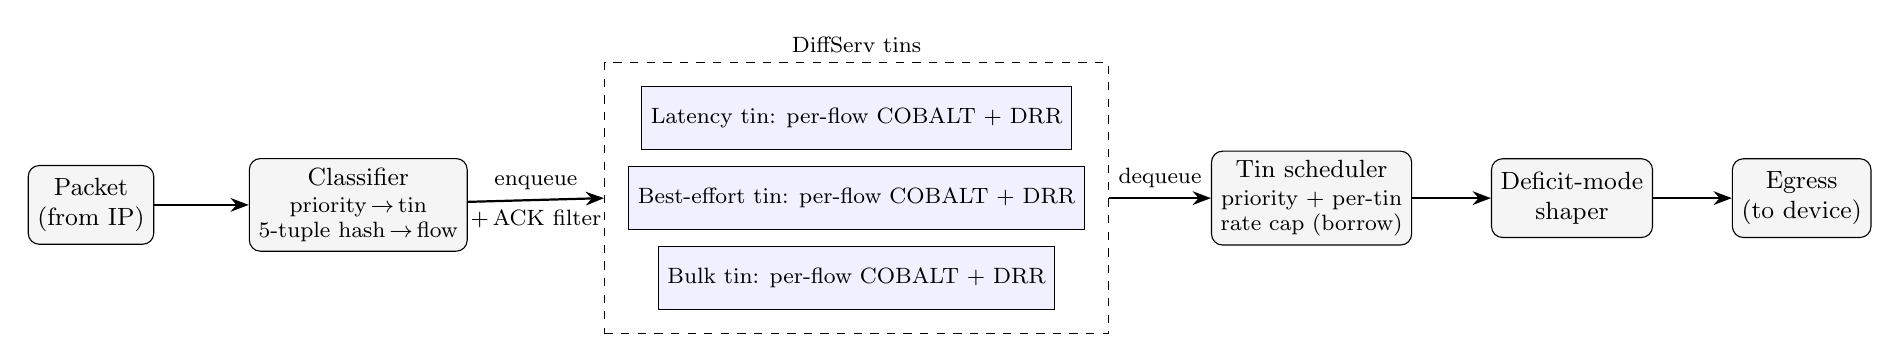
\begin{tikzpicture}[
  >=Stealth, node distance=10mm,
  box/.style={draw,rounded corners,align=center,minimum height=10mm,font=\small,fill=gray!8},
  tin/.style={draw,align=center,minimum width=46mm,minimum height=8mm,font=\footnotesize,fill=blue!6}]
\node[box] (in) {Packet\\(from IP)};
\node[box,right=12mm of in] (cls) {Classifier\\[-1pt]{\footnotesize priority\,$\to$\,tin}\\[-2pt]{\footnotesize 5-tuple hash\,$\to$\,flow}};
\node[tin,right=22mm of cls,yshift=11mm] (t0) {Latency tin: per-flow COBALT + DRR};
\node[tin,below=2mm of t0] (t1) {Best-effort tin: per-flow COBALT + DRR};
\node[tin,below=2mm of t1] (t2) {Bulk tin: per-flow COBALT + DRR};
\node[draw,dashed,inner sep=3mm,fit=(t0)(t1)(t2),label=above:{\footnotesize DiffServ tins}] (tins) {};
\node[box,right=16mm of t1] (sched) {Tin scheduler\\[-1pt]{\footnotesize priority + per-tin}\\[-2pt]{\footnotesize rate cap (borrow)}};
\node[box,right=10mm of sched] (shaper) {Deficit-mode\\shaper};
\node[box,right=10mm of shaper] (out) {Egress\\(to device)};
\draw[->,thick] (in) -- (cls);
\draw[->,thick] (cls) -- node[above,font=\footnotesize]{enqueue} node[below,font=\footnotesize]{+\,ACK filter} (tins.west);
\draw[->,thick] (tins.east) -- node[above,font=\footnotesize]{dequeue} (sched.west);
\draw[->,thick] (sched) -- (shaper);
\draw[->,thick] (shaper) -- (out);
\end{tikzpicture}}
\caption{Architecture of the ns-3 \texttt{CakeQueueDisc}. On enqueue a packet is
classified to a DiffServ tin (from its socket priority) and to a flow within the
tin (by a set-associative hash); pure ACKs may be marked by the ACK filter. Each
tin holds per-flow COBALT queues scheduled by host-fair deficit round robin. On
dequeue the tin scheduler selects a tin by priority subject to per-tin rate caps
(borrowing idle capacity), the flow DRR selects a flow, and the deficit-mode
shaper paces the packet to the configured rate.}
\label{fig:arch}
\end{figure*}

\subsection{Deficit-mode shaper}
When the \texttt{Bandwidth} attribute is non-zero, dequeues are paced by a
virtual-clock shaper: a packet may leave only when simulation time reaches the
shaper's \emph{time-next-packet}, which is advanced after each transmission by
the time to serialise the packet (plus a configurable per-packet overhead) at
the configured rate. While throttling, the disc schedules a self wake-up,
mirroring ns-3's token bucket filter. Setting \texttt{Bandwidth} to zero
disables shaping (unlimited mode). An idle period resets the clock to the
current time so that a burst cannot follow idleness.

\subsection{Flow isolation}
Each tin classifies packets into a configurable number of flow queues using a
(optionally set-associative) hash of the packet, exactly as FQ-COBALT does.
Each flow queue is a \texttt{CobaltQueueDisc} instance, and flows are scheduled
with DRR over ``new'' and ``old'' flow lists. We reuse the existing COBALT
implementation unchanged, which both reduces code and ensures the per-flow AQM
behaviour matches the rest of ns-3.

\subsection{DiffServ tins with per-tin rate caps}
\label{sec:tins}
The \texttt{DiffServMode} attribute selects 1, 3, 4 or 8 tins (best-effort,
diffserv3, diffserv4, precedence). Packets are mapped to a tin from their
socket priority---which the IP layer derives from the DSCP field---through a
per-mode priority map, the same dependency-clean mechanism ns-3's \texttt{prio}
qdisc uses. When shaping is enabled, each tin runs \emph{its own} virtual-clock
shaper at its share of the bandwidth: the scheduler serves the highest-priority
tin that is ``due'', and if none is due it lets the least over-budget tin borrow
idle capacity (work conserving). This caps each tin to its rate share while
giving latency-sensitive tins lower delay. In unlimited mode there is no total
rate to apportion, so the scheduler falls back to priority plus weighted DRR.
Algorithm~\ref{alg:dequeue} states the shaping-mode dequeue procedure, and
Algorithm~\ref{alg:enqueue} gives the enqueue counterpart---tin classification,
lazy flow creation, the host-counter update (lines 4--7), and the ACK-filter
mark performed by \textproc{TryAckFilter}.

\begin{algorithm}[t]
\caption{CAKE dequeue with per-tin rate caps (shaping mode). $R$ is the
configured rate; $T.\mathit{rate}$ is a tin's rate share; $t_{\text{next}}$ and
$T.t_{\text{next}}$ are the global and per-tin shaper clocks.}
\label{alg:dequeue}
\begin{algorithmic}[1]
\State $now \gets \textproc{Now}()$
\If{$now < t_{\text{next}}$} \Comment{global shaper throttling}
  \State schedule wake-up at $t_{\text{next}}$; \Return $\bot$
\EndIf
\Loop
  \State $best \gets \bot$
  \For{tins $T$ in priority order} \Comment{prefer a tin that is due}
    \If{$\textproc{HasTraffic}(T) \wedge T.t_{\text{next}} \le now$}
      \State $best \gets T$; \textbf{break}
    \EndIf
  \EndFor
  \If{$best = \bot$} \Comment{none due: borrow idle capacity}
    \State $best \gets$ backlogged tin minimising $T.t_{\text{next}}$
  \EndIf
  \If{$best = \bot$} \textbf{return} $\bot$ \Comment{no backlog} \EndIf
  \State $p \gets \textproc{DequeueFlowDRR}(best)$ \Comment{host-fair DRR; lazy ACK drop}
  \If{$p \ne \bot$}
    \State $best.t_{\text{next}} \gets \max(now, best.t_{\text{next}}) + \textproc{TxTime}(p, best.\mathit{rate})$
    \State $t_{\text{next}} \gets \max(now, t_{\text{next}}) + \textproc{TxTime}(p, R)$
    \State \Return $p$
  \EndIf \Comment{tin drained: reconsider}
\EndLoop
\end{algorithmic}
\end{algorithm}

\begin{algorithm}[t]
\caption{CAKE enqueue. Flow hashing, lazy flow creation, and \textproc{CakeDrop}
on overflow are inherited from \textsc{FqCobalt}; the host-counter update
(lines 4--7) and the \textproc{TryAckFilter} subroutine are the CAKE-specific
additions. The mark set on line~24 is consumed lazily on dequeue by
\textproc{DequeueFlowDRR} of Algorithm~\ref{alg:dequeue}.}
\label{alg:enqueue}
\begin{algorithmic}[1]
\State $h \gets$ flow hash of $\mathit{item}$ \Comment{5-tuple or a packet filter}
\State $T \gets m_{\mathit{tins}}[\,\textproc{Priomap}[\textproc{SockPrio}(\mathit{item})]\,]$
\State $f \gets T.\mathit{flow}[h]$ \Comment{created lazily on miss}
\If{$f.\mathit{status} = \mathit{Inactive}$}
  \If{a host classifier is set}
    \State $(s, d) \gets \textproc{HostClassifier}(\mathit{item})$
    \State $f.\textproc{SetHosts}(s, d)$;\, $T.\mathit{srcCnt}[s]{\,+\!\!+}$;\, $T.\mathit{dstCnt}[d]{\,+\!\!+}$
  \EndIf
  \State $f.\mathit{status} \gets \mathit{NewFlow}$;\, $f.\mathit{deficit} \gets \textproc{GrantQuantum}(T, f)$
  \State append $f$ to $T.\mathit{newFlows}$
\EndIf
\State $f.\mathit{queue}.\textproc{Enqueue}(\mathit{item})$ \Comment{the flow's COBALT}
\If{ACK filtering is on and an ACK identifier is set}
  \State \Call{TryAckFilter}{$f, \mathit{item}$}
\EndIf
\If{$\textproc{Size}() > \textproc{MaxSize}()$} \textproc{CakeDrop}() \EndIf
\State \Return $\top$
\Statex
\Procedure{TryAckFilter}{$f, \mathit{item}$}
  \If{$\neg\,\textproc{AckIdentifier}(\mathit{item}, \mathit{ackNo})$}
    \State \Return \Comment{not a pure ACK}
  \EndIf
  \If{$f.\mathit{hasLastAck} \wedge \mathit{ackNo} \ge f.\mathit{lastAckNo}$}
    \State $f.\textproc{MarkFiltered}(f.\mathit{lastAckUid})$ \Comment{older ACK now redundant}
  \EndIf
  \State $f.\textproc{SetLastAck}(\mathit{item}.\mathit{uid}, \mathit{ackNo})$
\EndProcedure
\end{algorithmic}
\end{algorithm}

\subsection{ACK filtering}
\label{sec:ackfilter}
CAKE thins redundant pure TCP ACKs. Recognising a pure ACK requires parsing
TCP/IP headers, but ns-3's layering forbids the \texttt{traffic-control} module
from depending on the \texttt{internet} module where those header types live.
We therefore expose a callback, \texttt{SetAckIdentifier}, that returns whether
an item is a pure ACK and its acknowledgement number; the concrete TCP/IPv4
implementation is supplied by the \texttt{internet} module
(Section~\ref{sec:impl}). A second constraint is that ns-3's \texttt{Queue} API
removes only from the head, so we cannot splice a superseded ACK out of the
middle of a flow queue as Linux does. Instead we mark a superseded ACK and drop
it \emph{lazily} when it reaches the head at dequeue. The superseded ACK is
therefore never transmitted---the upstream bandwidth saving is realised---though
it briefly occupies queue space.

\subsection{Host fairness (triple isolation)}
When a host classifier is installed (\texttt{SetHostClassifier}), the model
additionally enforces fairness between hosts. Each flow's per-round DRR grant is
scaled by $1/\max(\text{srcHostLoad}, \text{dstHostLoad})$, where the host loads
are the numbers of active flows of the flow's source and destination hosts.
A host that opens many flows therefore cannot claim more than its fair share of
host-level bandwidth. As with ACK filtering, the host-key extractor is injected
through a callback so the model need not parse addresses itself.

\subsection{Module-boundary design pattern}
Two of CAKE's mechanisms---ACK filtering and host fairness---fundamentally need
header information that ns-3 keeps in \texttt{internet}-module types
(\texttt{Ipv4QueueDiscItem}, \texttt{TcpHeader}), which \texttt{traffic-control}
must not depend on. Rather than relocate CAKE or invert the dependency, we keep
all header parsing in injected callbacks. The \texttt{internet} module, which
already depends on \texttt{traffic-control}, supplies concrete realisations
(\texttt{MakeTcpAckIdentifier}, \texttt{MakeIpv4HostClassifier}). This mirrors
ns-3's existing use of socket-priority tags and packet filters and keeps the
core model dependency-clean.

\section{Implementation}
\label{sec:impl}

The model comprises about 1{,}300 lines in the \texttt{traffic-control} module
(\texttt{cake-queue-disc.\{h,cc\}}) plus roughly 120 lines of
\texttt{internet}-module helpers and 900 lines of unit tests. A flow
is represented by \texttt{CakeFlow} (a \texttt{QueueDiscClass} carrying its DRR
deficit, status, ACK-tracking and host keys); a tin is a small struct holding
its flow lists, set-associative hash state, per-tin shaper clock and rate, and
per-host active-flow counts.

The configuration surface is exposed as ns-3 attributes (\texttt{Bandwidth},
\texttt{DiffServMode}, \texttt{AckFilter}, \texttt{Overhead}, \texttt{UseEcn},
the COBALT \texttt{Interval}/\texttt{Target}, \texttt{Flows},
\texttt{EnableSetAssociativeHash}, \texttt{SetWays}). Installing CAKE is thus a
one-line use of the standard \texttt{TrafficControlHelper}; enabling ACK
filtering or host fairness in a real simulation is a single call passing the
\texttt{internet}-module callback.

The model is covered by eight unit tests exercising, respectively: single-flow
FIFO ordering; two-flow DRR; shaper pacing; unlimited-mode bypass; DiffServ tin
priority; ACK filtering (a superseded ACK is dropped while data and the newest
ACK survive); host fairness; and per-tin rate caps.

\section{Validation against Linux \texttt{sch\_cake}}
\label{sec:validation}

\paragraph{Methodology.} We compare the model against Linux \texttt{sch\_cake}
using Flent's \emph{rrul} (``Realtime Response Under Load'') test, which runs
four bulk TCP flows in each direction together with latency probes. The Linux
reference is produced on a single host using three network namespaces---a
client, a router and a server---in which the router shapes both directions with
\texttt{tc qdisc \dots\ cake} and the endpoints add the base RTT with
\texttt{netem}. An ns-3 scenario mirrors this topology (bidirectional bulk TCP
over a CAKE-shaped bottleneck with a UDP echo RTT probe), using large TCP socket
buffers so that the window---rather than CAKE---is never the bottleneck at high
bandwidth-delay product, matching Linux's buffer autotuning. A comparison script
runs the ns-3 scenario for each operating point, reads the Flent results, and
reports the relative error per metric; the testbed and comparison tooling are
released with the module so the validation is reproducible.

\paragraph{Results.} Table~\ref{tab:validation} reports seven operating points.
From 5 to 100~Mbit/s the model tracks Linux closely: aggregate throughput
agrees within about 10\% and the round-trip latency percentiles within 6\% (often
under 1\% at higher rates). In every case CAKE holds the loaded RTT within a few
milliseconds of the base RTT, the behaviour the discipline is designed for.
Figure~\ref{fig:cdf} compares the full loaded-RTT distributions at three
operating points: ns-3 reproduces the shape of the Linux distribution at every
rate, with Linux showing slightly heavier tails---most visibly at 100~Mbit/s,
where the capture contains a handful of high-latency outliers that the
deterministic simulator does not generate.

\begin{figure*}[t]
\centering
\resizebox{\textwidth}{!}{%
\begin{tikzpicture}
\begin{axis}[width=6cm,height=4cm,
  xlabel={Loaded RTT (ms)},ylabel={CDF},ymin=0,ymax=1,
  title={10 Mbit/s, 40 ms},
  legend pos=south east,legend style={font=\footnotesize,row sep=-2pt},
  label style={font=\footnotesize},tick label style={font=\footnotesize},
  title style={font=\small}]
\addplot[thick,blue] table[x=rtt,y=cdf] {cdf-linux-10-40.dat}; \addlegendentry{Linux \texttt{cake}}
\addplot[thick,red,dashed] table[x=rtt,y=cdf] {cdf-ns3-10-40.dat}; \addlegendentry{ns-3 CAKE}
\end{axis}
\end{tikzpicture}\hspace{2mm}%
\begin{tikzpicture}
\begin{axis}[width=6cm,height=4cm,
  xlabel={Loaded RTT (ms)},ymin=0,ymax=1,
  title={50 Mbit/s, 80 ms},yticklabels={},
  label style={font=\footnotesize},tick label style={font=\footnotesize},
  title style={font=\small}]
\addplot[thick,blue] table[x=rtt,y=cdf] {cdf-linux-50-80.dat};
\addplot[thick,red,dashed] table[x=rtt,y=cdf] {cdf-ns3-50-80.dat};
\end{axis}
\end{tikzpicture}\hspace{2mm}%
\begin{tikzpicture}
\begin{axis}[width=6cm,height=4cm,
  xlabel={Loaded RTT (ms)},ymin=0,ymax=1,
  title={100 Mbit/s, 20 ms},yticklabels={},
  label style={font=\footnotesize},tick label style={font=\footnotesize},
  title style={font=\small}]
\addplot[thick,blue] table[x=rtt,y=cdf] {cdf-linux-100-20.dat};
\addplot[thick,red,dashed] table[x=rtt,y=cdf] {cdf-ns3-100-20.dat};
\end{axis}
\end{tikzpicture}}
\caption{Loaded round-trip-time CDFs at three operating points (Flent
\emph{rrul}, 4 bulk flows per direction). ns-3 CAKE reproduces the shape of the
Linux \texttt{sch\_cake} distribution at every rate. At 100~Mbit/s the Linux
capture contains a small number of high-latency outliers visible in the right
tail; the deterministic ns-3 simulation does not reproduce them.}
\label{fig:cdf}
\end{figure*}

\begin{table}[t]
\caption{ns-3 CAKE vs.\ Linux \texttt{sch\_cake} (Flent \emph{rrul}, 4 flows per
direction). Throughput is the aggregate per direction; RTT is the loaded
round-trip time. ns-3 / Linux.}
\label{tab:validation}
\small
\begin{tabular}{@{}lcccc@{}}
\toprule
Point & Down (Mbit/s) & Up (Mbit/s) & RTT p50 (ms) & RTT p99 (ms)\\
\midrule
1/40    & 0.6 / 0.9   & 0.5 / 0.9   & 48.7 / 61.3 & 71.6 / 90.3\\
5/40    & 4.3 / 4.6   & 4.2 / 4.6   & 43.7 / 44.4 & 49.5 / 51.1\\
10/40   & 8.7 / 9.3   & 8.6 / 9.4   & 41.4 / 42.2 & 43.5 / 45.7\\
20/100  & 16.8 / 18.1 & 16.8 / 18.1 & 100.7 / 101.0 & 101.7 / 103.0\\
50/80   & 44.4 / 44.7 & 42.1 / 45.8 & 80.3 / 80.5 & 80.7 / 81.3\\
100/20  & 93.2 / 93.1 & 93.3 / 93.1 & 20.2 / 20.6 & 20.3 / 23.0\\
100/80  & 85.7 / 89.0 & 85.7 / 88.8 & 80.2 / 80.6 & 80.3 / 82.2\\
\bottomrule
\end{tabular}
\end{table}

\begin{figure}[t]
\centering
\begin{tikzpicture}
\begin{axis}[width=0.44\columnwidth,height=3.8cm,
  xlabel={Linux (Mbit/s)},ylabel={ns-3 (Mbit/s)},title={Throughput},
  xmin=0,ymin=0,xmax=100,ymax=100,
  label style={font=\footnotesize},tick label style={font=\footnotesize},
  title style={font=\small,yshift=-1ex}]
\addplot[no markers,dashed,domain=0:100] {x};
\addplot[only marks,mark=*,mark size=1.5pt] table[x=linux,y=ns3] {validation-thr.dat};
\end{axis}
\end{tikzpicture}\hfill
\begin{tikzpicture}
\begin{axis}[width=0.44\columnwidth,height=3.8cm,
  xlabel={Linux (ms)},ylabel={ns-3 (ms)},title={RTT p99},
  xmin=0,ymin=0,xmax=110,ymax=110,
  label style={font=\footnotesize},tick label style={font=\footnotesize},
  title style={font=\small,yshift=-1ex}]
\addplot[no markers,dashed,domain=0:110] {x};
\addplot[only marks,mark=*,mark size=1.5pt] table[x=linux,y=ns3] {validation-rtt.dat};
\end{axis}
\end{tikzpicture}
\caption{Agreement between ns-3 CAKE and Linux \texttt{sch\_cake} across the seven
operating points of Table~\ref{tab:validation}: aggregate downstream throughput
(left) and loaded RTT 99th percentile (right). The dashed line is $y=x$ (perfect
agreement); points on the diagonal indicate a match. All points lie on the
diagonal except the 1~Mbit/s case (lower-left), which the model under-serves.}
\label{fig:validation}
\end{figure}

\paragraph{A low-rate limitation.} The 1~Mbit/s point is the exception: the
model delivers less throughput (0.6 vs.\ 0.9~Mbit/s) \emph{and} lower latency
(p50 49 vs.\ 61~ms) than Linux. The two together indicate over-dropping. The
cause is concrete: our per-flow COBALT uses a fixed 5~ms target, but at
1~Mbit/s a single 1500-byte packet takes about 12~ms to serialise---longer than
the target---so the standing-queue delay always exceeds the target and the AQM
drops too aggressively. Linux CAKE avoids this by scaling its CoDel target with
the configured rate. Making the target rate-adaptive is the clearest avenue to
close this gap (Section~\ref{sec:future}); we report the divergence rather than
hide it because it is exactly the kind of behaviour a validated model should
surface.

\section{Evaluation}
\label{sec:eval}

The evaluation exercises one CAKE mechanism at a time so that each headline
behaviour can be attributed to a specific feature. We first place CAKE among
ns-3's existing AQMs on a shared bottleneck (Table~\ref{tab:aqm},
Figure~\ref{fig:aqm}); we then turn on the integrated shaper and show it
controls bufferbloat end-to-end; we use unit-scale tests to exhibit host
fairness and per-tin rate caps; and we finally validate ACK filtering against
Linux on an asymmetric uplink (Table~\ref{tab:ack}). Unless stated otherwise the
TCP flows are Cubic with large socket buffers (so that the window is not the
binding constraint), the point-to-point device's own queue is kept small (so
that the queue disc under test, not the device, is the buffer), and four bulk
flows share the bottleneck alongside a sparse UDP probe that measures the
latency-under-load.

\paragraph{CAKE among ns-3 AQMs.} To place the model in context we run a single
bottleneck (4 bulk TCP flows, a sparse UDP latency probe, the device's own queue
kept small so the qdisc is the buffer) and compare CAKE against ns-3's
FQ-CoDel, FQ-COBALT, PIE and the default \texttt{pfifo\_fast}, all on the same
10~Mbit/s, 40~ms link (here CAKE runs in unlimited mode so all disciplines see
the same link-rate bottleneck). Table~\ref{tab:aqm} shows the canonical
bufferbloat picture: the flow-queueing AQMs (CAKE, FQ-CoDel, FQ-COBALT) hold the
probe's latency near the base RTT with good fairness; PIE controls delay but,
lacking flow isolation, gives the probe higher latency and lower fairness; and
the unmanaged FIFO bloats to nearly 400~ms. As expected, CAKE in unlimited mode
matches FQ-COBALT exactly, confirming that its flow-isolation core reuses that
machinery faithfully. Figure~\ref{fig:aqm} extends the comparison across
bottleneck rates: the flow-queueing AQMs keep the probe near the base RTT from
10 to 100~Mbit/s, while the FIFO's bloat, though it shrinks as the rate rises,
remains an order of magnitude larger at 10~Mbit/s. PIE controls latency
comparably but under-delivers throughput at 100~Mbit/s (68 vs.\ 97~Mbit/s for
the flow-queueing disciplines).

\begin{table}[t]
\caption{AQM comparison on a 10~Mbit/s, 40~ms bottleneck (4 flows). Latency is
the sparse probe's mean one-way delay.}
\label{tab:aqm}
\small
\begin{tabular}{@{}lcccc@{}}
\toprule
Qdisc & Thrpt (Mbit/s) & Jain & Latency (ms) & Drops\\
\midrule
CAKE        & 8.6 & 0.99 & 24.4  & 168\\
FQ-CoDel    & 9.2 & 0.98 & 24.6  & 159\\
FQ-COBALT   & 8.6 & 0.99 & 24.4  & 168\\
PIE         & 9.1 & 0.94 & 35.5  & 234\\
pfifo\_fast & 9.6 & 0.99 & 396.8 & 0\\
\bottomrule
\end{tabular}
\end{table}

\begin{figure}[t]
\centering
\begin{tikzpicture}
\begin{axis}[width=0.92\columnwidth,height=4.8cm,
  xlabel={Bottleneck rate (Mbit/s)},ylabel={Latency under load (ms)},
  ymode=log,xtick={10,50,100},
  legend pos=north east,legend style={font=\footnotesize,row sep=-2pt},
  label style={font=\small},tick label style={font=\footnotesize},
  mark size=2pt]
\addplot table[x=rate,y=PfifoFast] {aqm-latency.dat}; \addlegendentry{pfifo\_fast}
\addplot table[x=rate,y=Pie] {aqm-latency.dat}; \addlegendentry{PIE}
\addplot table[x=rate,y=FqCoDel] {aqm-latency.dat}; \addlegendentry{FQ-CoDel}
\addplot table[x=rate,y=Cake] {aqm-latency.dat}; \addlegendentry{CAKE}
\end{axis}
\end{tikzpicture}
\caption{Latency under load vs.\ bottleneck rate (40~ms base RTT, 4 bulk flows,
sparse UDP probe; log scale). CAKE and FQ-CoDel hold the probe near the base
one-way delay at every rate (FQ-COBALT is identical to CAKE and is omitted),
whereas the unmanaged FIFO bloats severely---nearly 400~ms at 10~Mbit/s.}
\label{fig:aqm}
\end{figure}

\paragraph{Shaping and bufferbloat control.} A second example uses CAKE as the
bottleneck rather than just as an AQM: CAKE is installed as a $10$~Mbit/s
shaper on a $100$~Mbit/s link, with three long-lived Cubic flows and a $22$~ms
base RTT. Table~\ref{tab:bufferbloat} reports the steady-state result of a
$30$~s run. The deficit-mode shaper holds the aggregate at $9.01$~Mbit/s---
about $90\%$ of the configured rate, the remainder ceded to TCP backoff after
$483$ COBALT drops over the run---and the three flows share that aggregate
with a Jain's-fairness index of $0.995$. The mean one-way delay sits at
$\approx 18.6$~ms, only about $7$~ms above the $11$~ms base one-way
propagation: COBALT's $5$~ms target is honoured under saturation, and CAKE
prevents the standing queue from growing. The mechanism is the same one the
validation experiment of Section~\ref{sec:validation} exercises---just with
the shaper, rather than the link, as the bottleneck.

\begin{table}[t]
\caption{CAKE as a $10$~Mbit/s shaper on a $100$~Mbit/s link: three long-lived
Cubic flows, $22$~ms base RTT, $30$~s run. Throughput is FlowMonitor's
aggregate; ``mean delay'' is FlowMonitor's per-flow one-way delay (base one-way
is $11$~ms).}
\label{tab:bufferbloat}
\small
\begin{tabular}{@{}lcc@{}}
\toprule
Flow & Throughput (Mbit/s) & Mean one-way delay (ms)\\
\midrule
1         & 3.19 & 18.55\\
2         & 2.71 & 18.81\\
3         & 3.11 & 18.56\\
\midrule
Aggregate / mean & 9.01 & 18.64\\
\bottomrule
\end{tabular}
\end{table}

\paragraph{Host fairness.} The host-fairness unit test backlogs three flows that
share a single tin: two from source host~A (towards two different destinations)
and one from source host~B. With plain flow fairness host~A's two flows out-serve
host~B's single flow by roughly $2{:}1$ (the test asserts $\textit{A}_{\text{flow}}>1.4\,\textit{B}_{\text{flow}}$). When a host classifier is
installed and host fairness is enabled, each flow's per-round DRR grant is
scaled by $1/\max(\textit{srcHostLoad}, \textit{dstHostLoad})$, and the two
hosts obtain approximately equal shares ($|\textit{A}-\textit{B}|<0.3\textit{B}$,
i.e.\ the asserted ratio collapses to $1{:}1$). This is the feature that most
distinguishes CAKE from ns-3's existing flow-queueing AQMs, which give a busy
host more bandwidth simply by opening more flows.

\paragraph{Per-tin rate caps.} A further test, with shaping enabled and both a
high-priority small-share tin (latency) and a low-priority large-share tin (best
effort) backlogged, confirms that the best-effort tin out-serves the
rate-capped latency tin (its share is larger), while a single backlogged tin
borrows the entire link---the work-conserving behaviour described in
Section~\ref{sec:tins}.

\paragraph{ACK filtering on asymmetric links.} ACK filtering targets paths whose
uplink is far slower than their downlink. To both demonstrate the feature and
validate it against Linux, we run Flent's \emph{rrul} workload (four downloads
plus four uploads) over a 50/1~Mbit/s asymmetric link in both ns-3 and Linux
\texttt{sch\_cake}, with the CAKE ACK filter toggled on and off. The four
uploads share the 1~Mbit/s uplink with the four downloads' ACK streams, so the
uplink is the contended resource. Table~\ref{tab:ack} reports the resulting
downstream throughput and loaded 99th-percentile RTT for each combination. Two
findings stand out. First, \emph{ACK filtering is reproduced and validated}:
with the filter enabled the ns-3 model agrees with Linux to within $\sim$1\% on
both throughput and tail latency ($42.9$ vs.\ $42.8$~Mbit/s; $70.9$ vs.\
$70.0$~ms p99), and both systems show the canonical throughput uplift the
feature was designed to deliver (Linux: $33{\to}43$~Mbit/s, $+30\%$; ns-3:
$38{\to}43$~Mbit/s, $+11\%$) by dropping roughly $40{,}000$ redundant ACKs over
the 30~s run. Second, the \emph{unfiltered baseline diverges}: ns-3's loaded
RTT without the filter rises noticeably higher than Linux's ($p99{=}182$ vs.\
$66$~ms), pointing to a difference in how the two implementations cope with
ACKs piling up behind upload data on a saturated uplink. The configuration
operators actually deploy---ACK filtering enabled---is the one we reproduce
most precisely.

\begin{table}[t]
\caption{Validation of CAKE ACK filtering on a 50/1~Mbit/s asymmetric link
under Flent \emph{rrul} (4~down + 4~up, downstream metrics).}
\label{tab:ack}
\small
\begin{tabular}{@{}llcc@{}}
\toprule
Configuration & System & Down (Mbit/s) & RTT p99 (ms)\\
\midrule
ack filter \emph{on}  & ns-3 CAKE          & 42.9 & 70.9\\
                      & Linux \texttt{cake} & 42.8 & 70.0\\
ack filter \emph{off} & ns-3 CAKE          & 38.5 & 182.3\\
                      & Linux \texttt{cake} & 33.0 & 66.2\\
\bottomrule
\end{tabular}
\end{table}

\section{Limitations and Future Work}
\label{sec:future}

The model is faithful across a wide operating range but is not yet complete.
First, as Section~\ref{sec:validation} shows, the per-flow CoDel target is fixed
rather than scaled to the configured rate as Linux CAKE does; making it
rate-adaptive would close the low-rate gap. Second, ACK filtering removes
superseded ACKs lazily (at dequeue) rather than in place, a consequence of the
head-only \texttt{Queue} API; an extended queue interface would allow exact
in-place removal. Third, the provided header-inspection callbacks handle IPv4
TCP only; IPv6 support is a small addition. Fourth, the validation covers seven
operating points and a single topology; a broader sweep (more rates, RTTs,
flow counts, and asymmetric links that exercise ACK filtering) would strengthen
the comparison, and the released campaign tooling is designed for exactly that.
Finally, the deterministic ns-3 simulator does not, by construction, reproduce
the system-level jitter (kernel scheduling, NIC interrupts) that produces the
high-latency outliers visible in Linux at 100~Mbit/s in Figure~\ref{fig:cdf};
this is a fidelity boundary of the simulator rather than of CAKE itself, but it
is worth flagging when interpreting tail-latency results.

\section{Conclusion}
\label{sec:conclusion}

We have presented the first ns-3 model of CAKE, implemented in the
\texttt{traffic-control} module by reusing the existing COBALT AQM and adding
CAKE's shaper, DiffServ tins with per-tin rate caps, ACK filtering and host-fair
triple isolation. A dependency-clean callback design keeps the model free of
transport/network header types while still supporting header-aware features.
Validated against Linux \texttt{sch\_cake} with Flent's \emph{rrul} test, the
model agrees within roughly 10\% on throughput and 6\% on latency percentiles
from 5 to 100~Mbit/s. The validation also surfaces two honest fidelity
boundaries: at very low rates the fixed CoDel target over-drops where Linux
would adapt, and at high rates the CDF's right tail in the Linux capture
contains a handful of outliers that a deterministic simulator does not
generate---a useful reminder that faithful AQM behaviour and real-system
jitter are separate axes of fidelity. Both observations point to concrete next
steps. The model, its unit tests, runnable examples and a reproducible
validation harness are released for inclusion in ns-3.\footnote{Sources for
the model, validation harness, and committed Linux references are on the
\texttt{ns3-summer-2026} branch; reviewers can start from the guided
README at
\url{https://github.com/Haoyu2/ns3/blob/ns3-summer-2026/README.md}.}

\bibliographystyle{ACM-Reference-Format}
\bibliography{references}

\end{document}
